%% The first command in your LaTeX source must be the \documentclass command.
\documentclass[sigconf]{acmart}

%% \BibTeX command to typeset BibTeX logo in the docs
\AtBeginDocument{%
  \providecommand\BibTeX{{%
    \normalfont B\kern-0.5em{\scshape i\kern-0.25em b}\kern-0.8em\TeX}}}

%% Rights management information.  This information is sent to you
%% when you complete the rights form.  These commands have SAMPLE
%% values in them; it's your responsibility as an author to replace
%% the commands and values with those provided to you when you
%% complete the rights form.
\setcopyright{acmcopyright}
\copyrightyear{2023}
\acmYear{2023}
\acmDOI{XXXXXXX.XXXXXXX}

%% These commands are for a~PROCEEDINGS abstract or paper.
\acmConference[WWW '23]{The Web Conference 2023}{April 30 -- May 4,
  2023}{Austin, TX}
%
%  Uncomment \acmBooktitle if th title of the proceedings is different
%  from ``Proceedings of ...''!
%
%\acmBooktitle{Woodstock '18: ACM Symposium on Neural Gaze Detection,
%  June 03--05, 2018, Woodstock, NY} 
\acmPrice{15.00}
\acmISBN{978-1-4503-XXXX-X/18/06}

\usepackage{graphicx}
\usepackage{enumitem}
\usepackage{float}

\newlist{questions}{enumerate}{2}
\setlist[questions,1]{label=RQ\arabic*.,ref=RQ\arabic*}
\setlist[questions,2]{label=(\alph*),ref=\thequestionsi(\alph*)}

%%
%% end of the preamble, start of the body of the document source.
\begin{document}

%%
%% The "title" command has an optional parameter,
%% allowing the author to define a~"short title" to be used in page headers.
\title{The Capable Web}

%%
%% The "author" command and its associated commands are used to define
%% the authors and their affiliations.
%% Of note is the shared affiliation of the first two authors, and the
%% "authornote" and "authornotemark" commands
%% used to denote shared contribution to the research.
\author{Thomas Steiner}
\email{steiner.thomas@gmail.com}
\affiliation{%  
  \streetaddress{Haselnussweg 3/1}
  \city{Reutlingen}  
  \country{Germany}
  \postcode{72770}
}

%%
%% By default, the full list of authors will be used in the page
%% headers. Often, this list is too long, and will overlap
%% other information printed in the page headers. This command allows
%% the author to define a~more concise list
%% of authors' names for this purpose.
% \renewcommand{\shortauthors}{Trovato and Tobin, et al.}

%%
%% The abstract is a~short summary of the work to be presented in the
%% article.
\begin{abstract}
  In this paper, I discuss arguments in favor and in disfavor of building for the Web. I look at three extraordinary examples of apps built for the Web, and analyze reasons their creators provided for doing so. In continuation, I look at the decline of interest in cross-platform app frameworks with the exception of Flutter, which leads me to the two research questions (i) "Why do people not fully bet on PWA" and (ii) "Why is Flutter so popular". My hypothesis for why developers don't more frequently set on the Web is that in many cases they (or their non-technical reporting lines) don't realize how powerful it has become. To counter that, I introduce a~Web app and a~browser extension that demonstrate the Web's capabilities.
\end{abstract}

%%
%% The code below is generated by the tool at http://dl.acm.org/ccs.cfm.
%% Please copy and paste the code instead of the example below.
%%
\begin{CCSXML}
<ccs2012>
<concept>
<concept_id>10002951.10003260.10003300.10003302</concept_id>
<concept_desc>Information systems~Browsers</concept_desc>
<concept_significance>500</concept_significance>
</concept>
</ccs2012>
\end{CCSXML}

\ccsdesc[500]{Information systems~Browsers}

%%
%% Keywords. The author(s) should pick words that accurately describe
%% the work being presented. Separate the keywords with commas.
\keywords{Progressive Web Apps, Project Fugu, browser APIs, Web extensions}

%%
%% This command processes the author and affiliation and title
%% information and builds the first part of the formatted document.
\maketitle

\section{Introduction}

If you want to build an app, you have several ways of doing it. You can build a~platform-specific app for the platforms you care about, for example, Windows, Android, and iOS. In which case you would build three apps. You can also build a~(Progressive) Web App, possibly in addition to platform-specific apps. Alternatively, you can choose a~cross-platform framework such as Electron.js\footnote{\url{https://www.electronjs.org/}} or Ionic\footnote{\url{https://ionicframework.com/}} that promises to let you write once and run anywhere. Let me begin by walking you through three extraordinary examples of apps whose makers chose to also build for the Web, apart from building platform-specific apps.

\subsection{Beacon cases for the Web's abilities}

\subsubsection{Photoshop}

I always saw Photoshop as one of the last bastions of high quality apps that supposedly would never make it to the Web platform. This last bastion has finally fallen. With Photoshop,\footnote{\url{https://web.dev/ps-on-the-web/}} Adobe, together with Chromium engineering, has managed to get a~beta version of Photoshop running in the browser (see \autoref{fig:photoshop}) that can serve as the new beacon showcase of what is possible on the Web. In it, you can try out the commenting workflow and test some early Photoshop editing features Adobe is piloting on the Web. You and your collaborators can now open and view Photoshop cloud documents in the browser, provide feedback, and make basic edits. All from the Web without having to download the full Photoshop app for your specific operating system.

\begin{figure}[b]
    \centering
    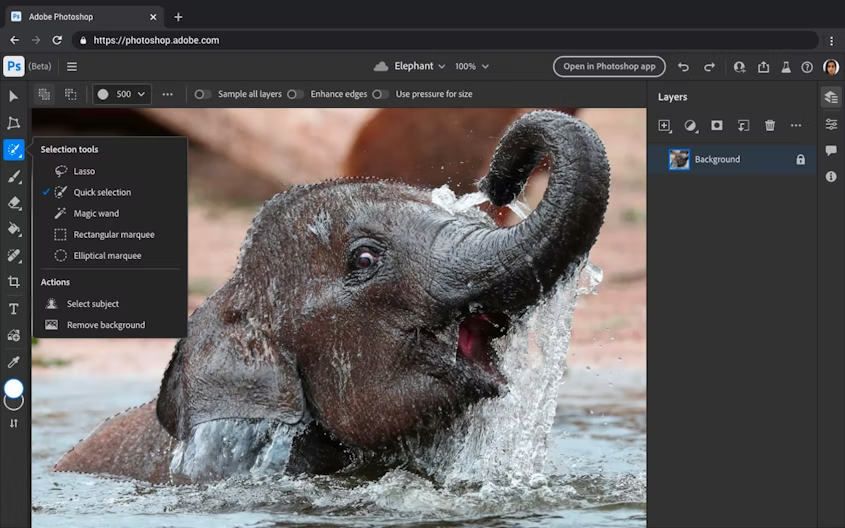
\includegraphics[width=\columnwidth]{photoshop.png}
\caption{Photoshop on the Web}
    \label{fig:photoshop}
    \Description{Screenshot of the Photoshop app.}
\end{figure}

\subsubsection{Visual Studio Code}
Similarly, Microsoft has launched Visual Studio Code\footnote{\url{https://code.visualstudio.com/blogs/2021/10/20/vscode-dev}} on the Web (see \autoref{fig:vscode}), a~fully fledged, installable Web experience of its integrated development environment (IDE) that makes developing completely in the browser possible, including the option to open and edit files on the local file system.

\begin{figure}[t]
    \centering
    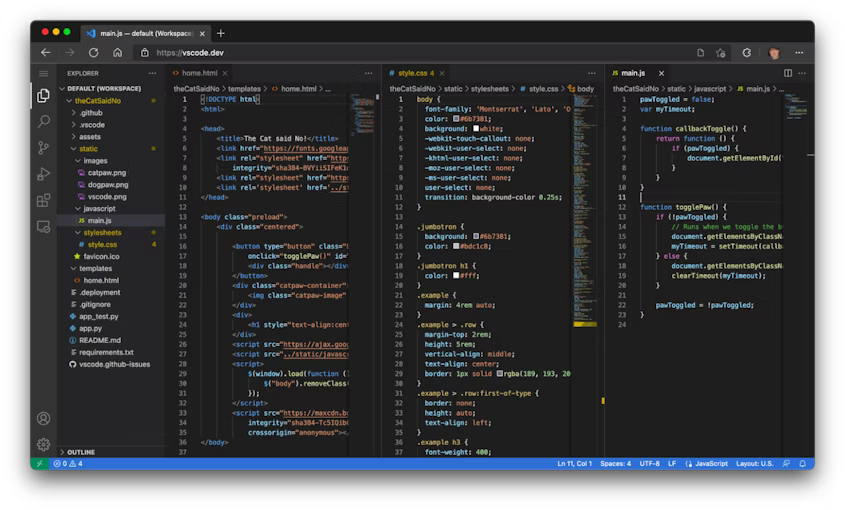
\includegraphics[width=0.9\columnwidth]{vscode.png}
    \caption{VS~Code on the Web}
    \label{fig:vscode}
    \Description{Screenshot of the Visual Studio Code app.}
\end{figure}

\subsubsection{Twitter}
Lastly Twitter—whose Progressive Web App (PWA) is largely seen as probably the best mainstream Progressive Web App\footnote{\url{https://www.thurrott.com/cloud/social/150171/}}—has used its responsive Web codebase for all platforms, mobile and desktop, via Web browsers.\footnote{\url{https://blog.twitter.com/engineering/en_us/topics/insights/2019/twitter-for-mac-is-coming-back}} On Windows, the PWA is the experience the company is confident enough to make the Twitter experience that you get when you install the app from the Microsoft Store\footnote{\url{https://blog.twitter.com/en_us/topics/product/2018/a-new-twitter-experience-on-windows}} (see \autoref{fig:twitter}).

\begin{figure}[t]
    \centering
    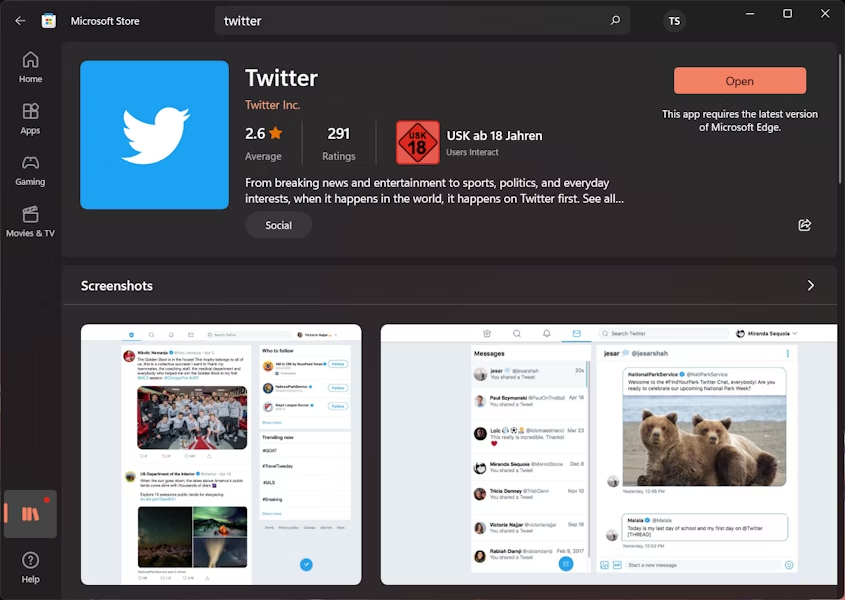
\includegraphics[width=0.8\columnwidth]{twitter.png}
    \caption{Twitter in the Microsoft Store}
    \label{fig:twitter}
    \Description{Screenshot of the Twitter app in the Microsoft Store.}
\end{figure}

\section{Linkability and universality: the Web's super powers}

\paragraph{Linkability}

All three companies, Adobe, Microsoft, and Twitter, in parallel with their Web apps, have well-established, platform-specific Windows, macOS, Android, iOS, and Linux versions of their apps Photoshop, Visual Studio Code, and Twitter respectively. So why did they build for the Web on top? The answer lies in its linkability and universality.

As Google's Thomas Nattestad put it: \textit{"The simple power of a~URL is that anyone can click it and instantly access it. All you need is a~browser. There is no need to install an application or worry about what operating system you are running on"}.\footnote{\url{https://web.dev/ps-on-the-web/}} According to Microsoft's Chris Dias, with Visual Studio Code for the Web, when working with GitHub \textit{"you can make quick edits, review PRs, and continue on to a~local clone"}.\footnote{\url{https://code.visualstudio.com/blogs/2021/10/20/vscode-dev}} The sole fact that you can share a~link to your work unlocks collaboration patterns that users have embraced and loved since the birth of apps such as Google Docs. Twitter, of course, lives and dies by its links. News sites regularly link to newsworthy tweets, which means \textit{"keeping it quick"}\footnote{\url{https://blog.twitter.com/engineering/en_us/topics/infrastructure/2019/progressively-enhancing-desktop-devices}} is core to ensuring people can get from an article straight into the app, where they can read or engage with the linked tweet.

\paragraph{Linkability of platform-specific apps}

While more ubiquitous on mobile, linking into a~platform-specific app from the Web on desktop is comparatively rare. On mobile (and macOS), this works via a~technology called Universal Links\footnote{\url{https://developer.apple.com/ios/universal-links/}} on iOS (and on macOS), and App Links\footnote{\url{https://developer.android.com/training/app-links/}} on Android. Platform-specific apps alternatively can rely on registered protocol schemes\footnote{\url{https://developer.apple.com/documentation/xcode/defining-a-custom-url-scheme-for-your-app}} such as \texttt{itms-apps:} for when you want to deep-link into the App Store app on macOS or iOS, or register your own custom schemes for your own apps. So while technically possible, linking into platform-specific apps is a~lot less flexible and requires more plumbing work than simply linking into a~Web app.

\paragraph{Universality}

Web applications are inherently universal. They run on whatever operating system is capable of running a~Web browser and they do not need to be compiled for each operating system separately. The same code base powers the application on all platforms. This doesn't mean that there are no compatibility issues—there are plenty actually—but there is a~solid, shared, increasing baseline\footnote{\url{https://web.dev/interop-2022/}} that all applications can build upon.

\section{The slow decline of interest in cross-platform app frameworks and the rise of Flutter}

The Web isn't the only platform that promises "write once, run anywhere". Cross-platform frameworks à la Electron.js do, too. With the Web becoming powerful enough to drive apps such as Photoshop that were thought to be impossible, we can, however, observe a~slow decline of interest in cross-platform desktop app frameworks such as Electron.js and NW.js,\footnote{\url{https://nwjs.io/}} and mobile app frameworks such as Cordova\footnote{\url{https://cordova.apache.org/}} or React Native;\footnote{\url{https://reactnative.dev/}} while at the same time there is an undeniable \textit{increase} of interest in Flutter.\footnote{\url{https://flutter.dev/}}

\paragraph{Google Trends stats}

The Google Trends chart\footnote{\url{https://goo.gle/google-trends-cross-platform-apps-frameworks}} in \autoref{fig:googletrends} shows the five frameworks side by side. While noting that this chart does show disambiguated \textit{topic trends} as detected by Google (as opposed to ambiguous \textit{search term trends}), it's clearly not an exact science.

\paragraph{Statista stats}

As shown in \autoref{fig:statista}, this trend is backed by data observed by Statista,\footnote{\url{https://www.statista.com/statistics/869224/}} according to which Flutter has passed React Native as the most popular framework.

\paragraph{StackOverflow stats}

StackOverflow statistics\footnote{\url{https://goo.gle/stackoverflow-cross-platform-apps-frameworks}} on tag usage also support this, as you can see in \autoref{fig:stackoverflow}. The underlying assumption of people actually using a~technology correlating with people asking questions about that technology on StackOverflow isn't beyond the realms of possibility.

\begin{figure}[H]
    \centering
    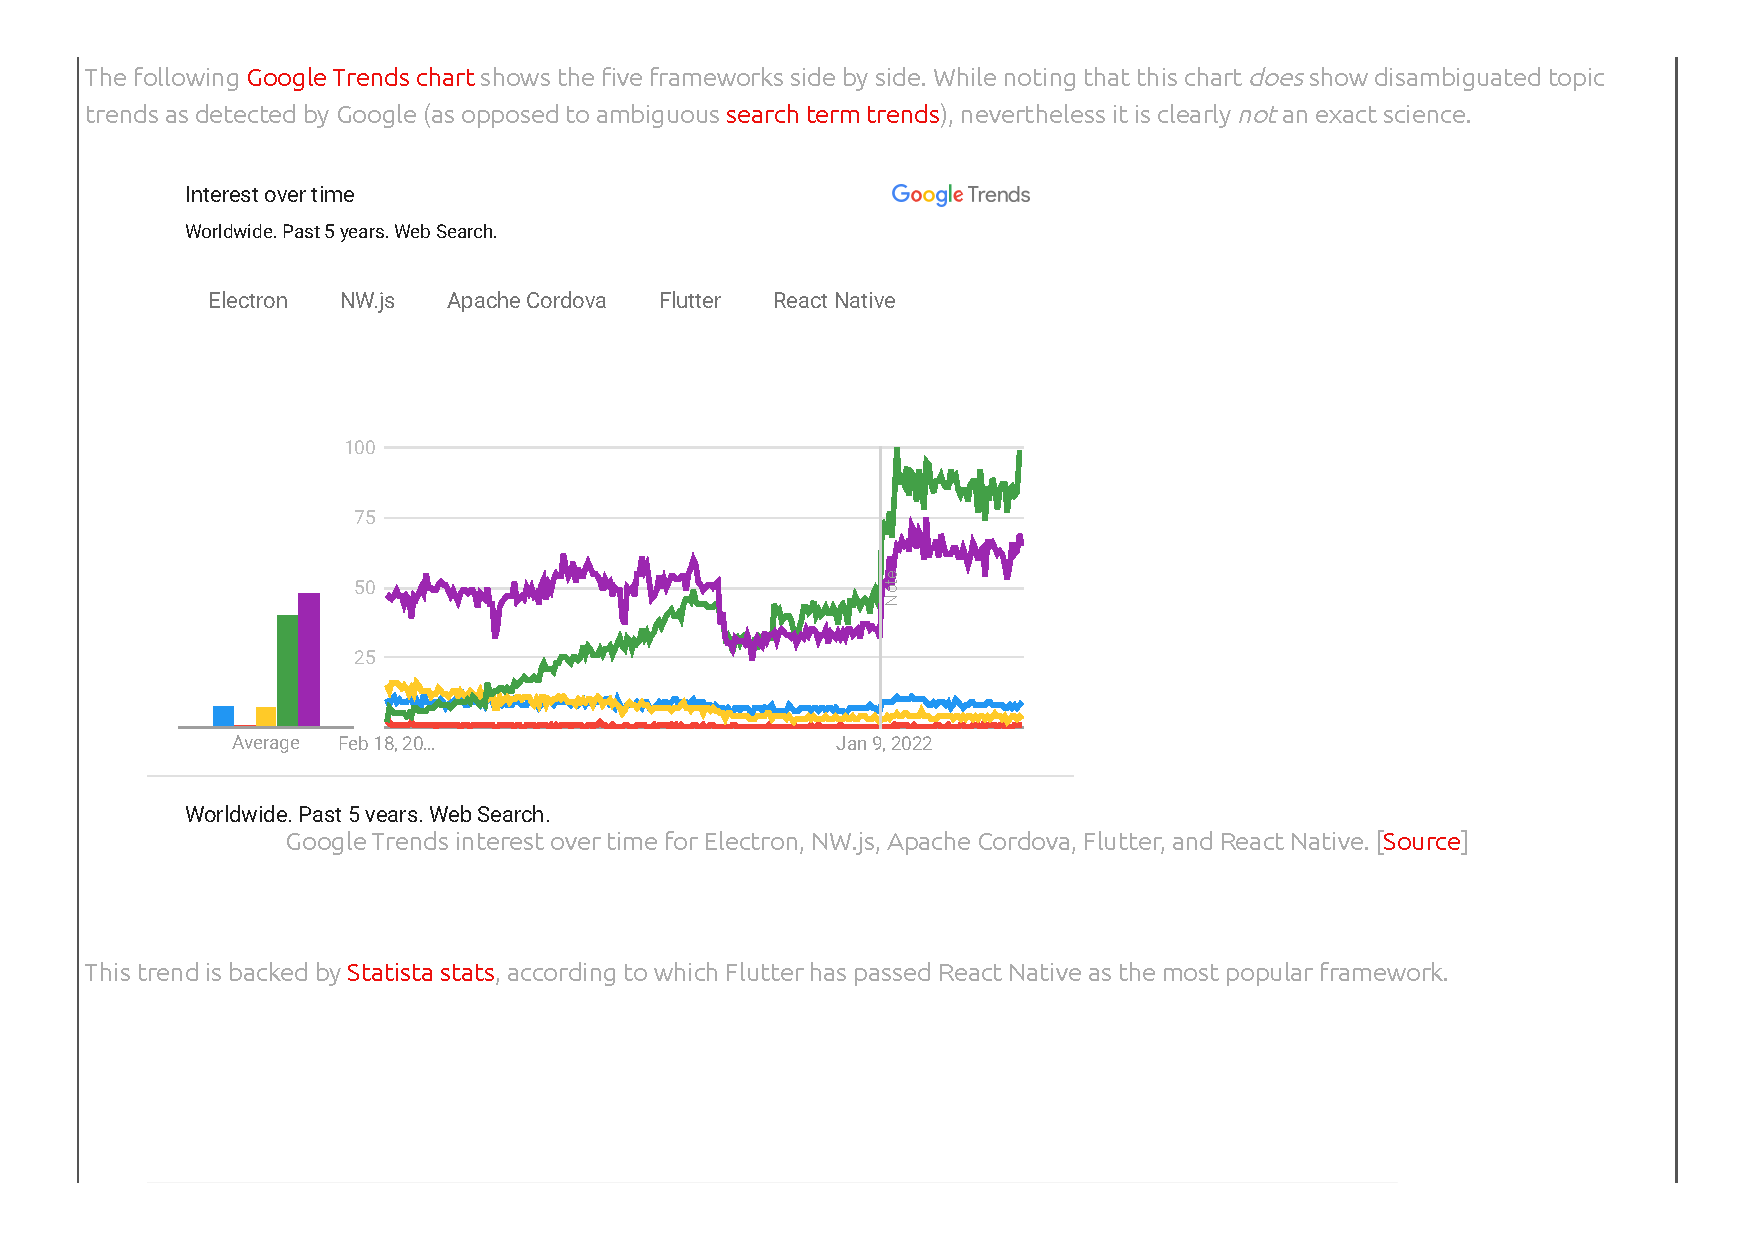
\includegraphics[clip, trim=3.5cm 8.2cm 12cm 4.5cm, width=\columnwidth]{Google Trends.pdf}
    \caption{Google Trends interest over time for Electron (blue), NW.js (red), Apache Cordova (yellow), Flutter (green), and React Native (purple)}
    \label{fig:googletrends}
    \Description{Google Trends interest over time for Electron, NW.js, Apache Cordova, Flutter, and React Native. The chart shows how interest in Flutter and React Native grows, with Flutter leading.}
\end{figure}

\begin{figure}[H]
    \centering
    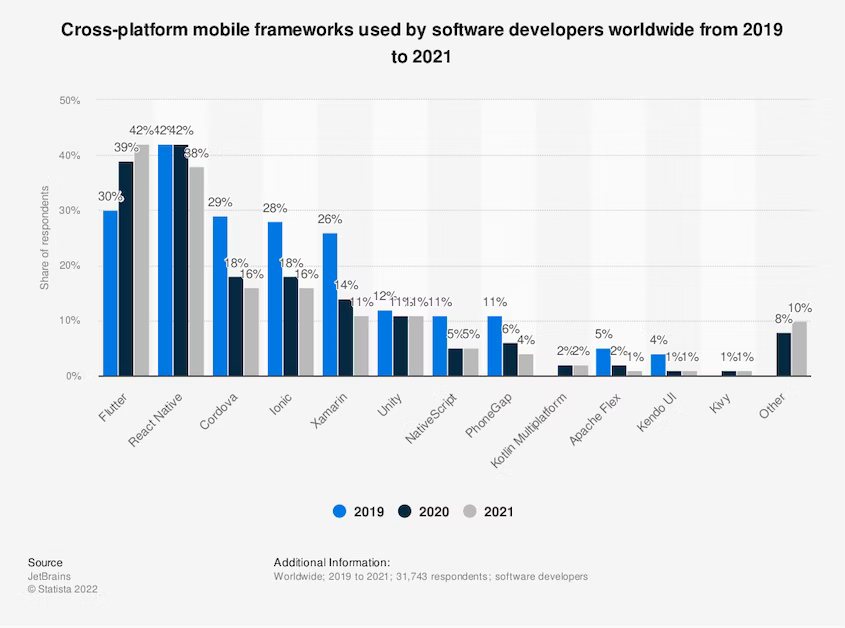
\includegraphics[width=\columnwidth]{statista.png}
    \caption{Cross-platform mobile frameworks used by software developers worldwide from 2019 to 2021}
    \label{fig:statista}
    \Description{Cross-platform mobile frameworks used by software developers worldwide from 2019 to 2021 showing how Flutter's usage grows in the observed period, all other frameworks' usages shrink.}
\end{figure}

\begin{figure}[H]
    \centering
    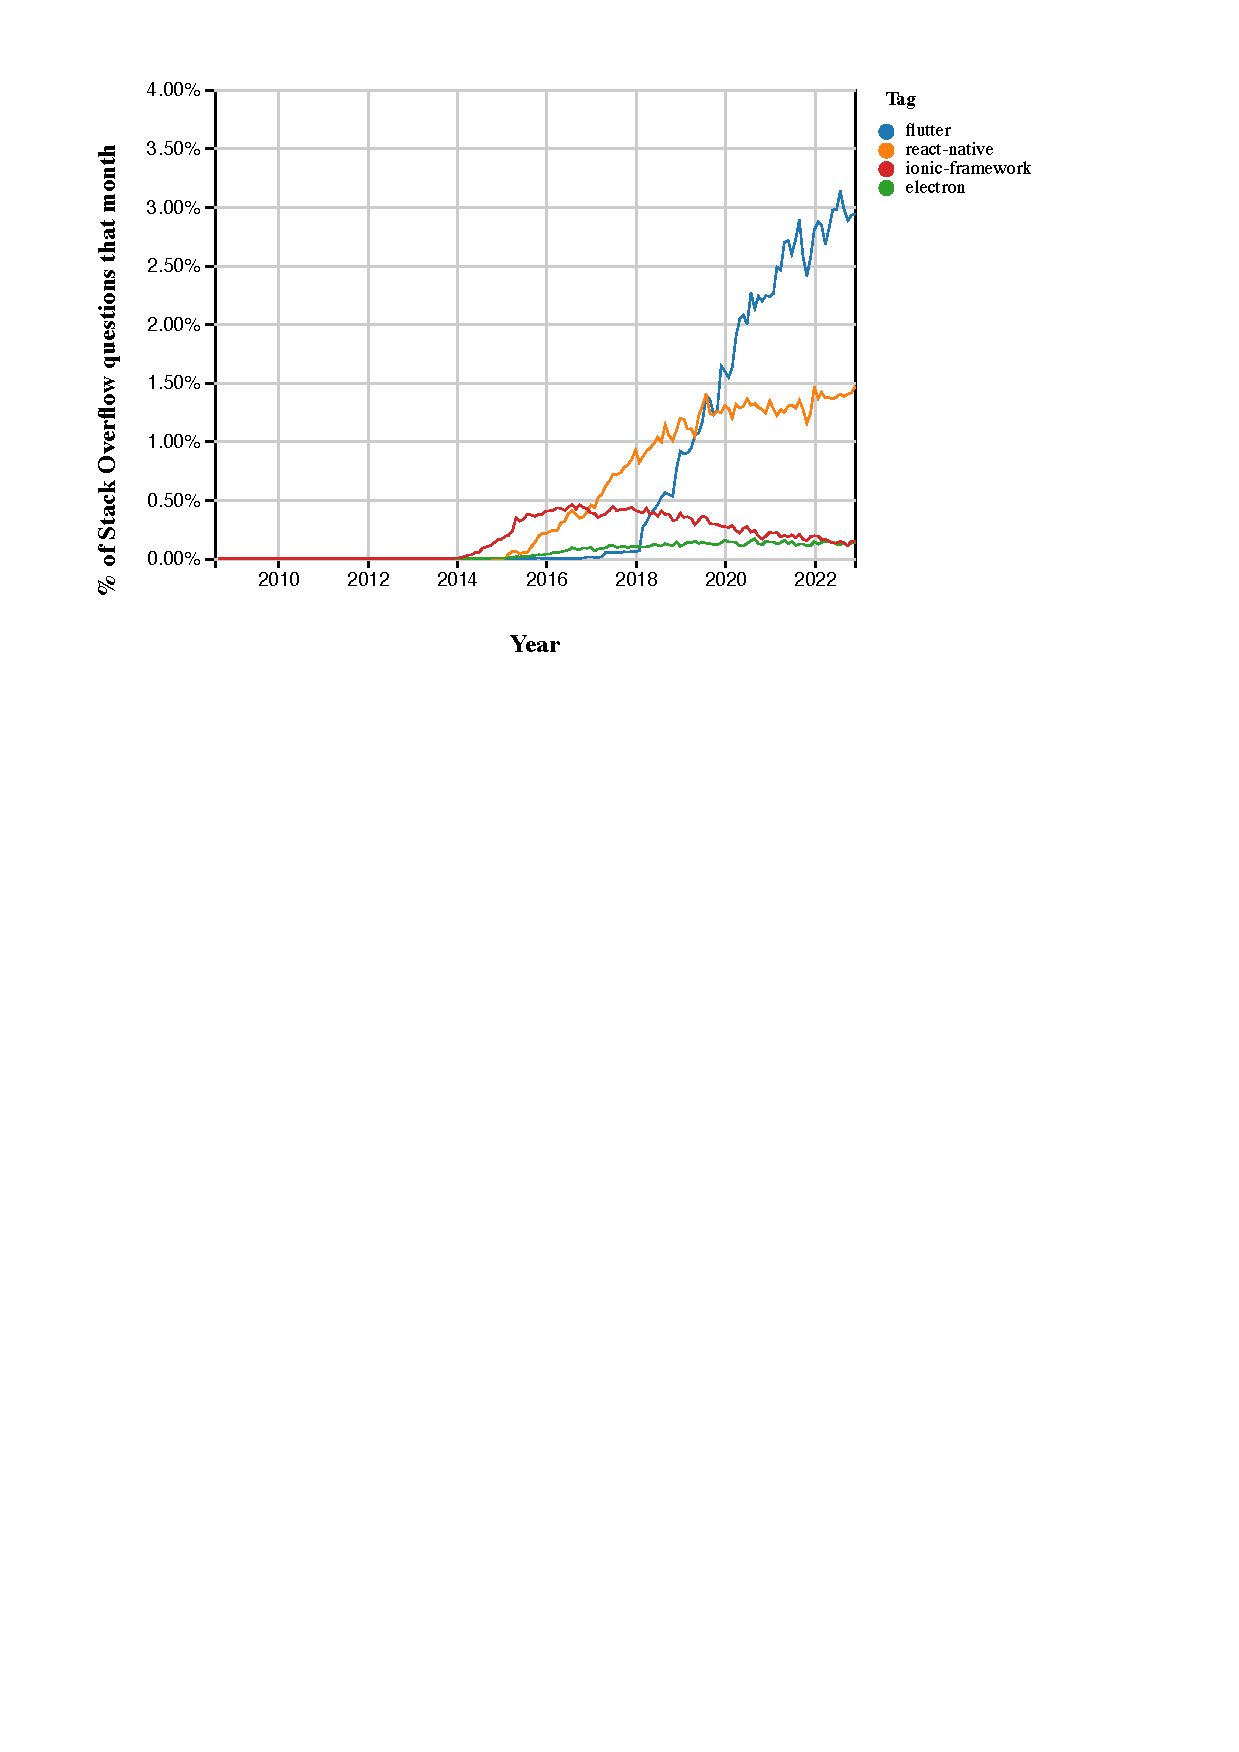
\includegraphics[clip, trim=1.5cm 18.2cm 3.5cm 1.25cm, width=\columnwidth]{stackoverflow.pdf}
    \caption{StackOverflow statistics on tag usage}
    \label{fig:stackoverflow}
    \Description{StackOverflow statistics on tag usage showing how the flutter tag goes through the roof.}
\end{figure}

\section{Research questions}

Given the examples of Photoshop, VS~Code, and Twitter, that show that it's indeed possible to build amazing applications on the Web, and given the Web's super powers of linkability and universality plus the decline in cross-platform app frameworks (except Flutter), two research questions come up:

\begin{questions}
    \item Why do people not fully bet on PWA?\label{itm:rq1}
    \item Why is Flutter so popular?\label{itm:rq2}    
\end{questions}

\section{Why do people not fully bet on PWA?}

For \ref{itm:rq1}, the answer is complex and manifold. I want to break it down into different sub-categories.

\subsection{Missing capabilities: aka the app gap}

Web applications still lack certain functionalities that platform-specific apps have. In the following paragraph, I list representative examples of such functionalities on different platforms.

First, it's impossible, even with an installed PWA, to obey the macOS user interface paradigm of having the app menu at the top of the screen.\footnote{\url{https://developer.apple.com/design/human-interface-guidelines/macos/menus/menu-bar-menus/}} It can easily be achieved with frameworks such as Electron.js via the \texttt{Menu}\footnote{\url{https://www.electronjs.org/docs/latest/api/menu}} class. (On the Web, the next best thing is Window Controls Overlay;\footnote{\url{https://web.dev/window-controls-overlay/}} getting support for app menus is tracked as \url{https://crbug.com/1295253}.) Another example is in-app purchases on macOS that can be handled via Electron's \texttt{inAppPurchase()} method.\footnote{\url{https://www.electronjs.org/docs/latest/tutorial/in-app-purchases}} (On the Web, the next best thing is the Digital Goods API,\footnote{\url{https://goo.gle/trusted-web-activity-receive-payments}} currently limited to Android and ChromeOS.) Installers are a~common way users have learned to install applications on Windows. With Electron.js, it's possible to create installers\footnote{\url{https://www.electronjs.org/docs/latest/api/auto-updater\#windows}} and make installed applications update automatically.\footnote{\url{https://www.electronjs.org/docs/latest/api/auto-updater}} (On the Web, Web Bundles\footnote{\url{https://web.dev/web-bundles/}} are the next best alternative in Chrome.) This list isn't exhaustive, and Electron.js is mentioned as a~representative app framework out of several.

\paragraph{How big a~challenge is this?}

There are undeniably a~number of capabilities that are missing from the Web. In many cases, they are "nice-to-have", but not necessarily required for a~still great experience. Carefully assess if a~capability can be seen as a~progressive enhancement. For an example of this approach, check out the article Progressively enhance your Progressive Web App.\footnote{\label{footnote:progressively-enhance}\url{https://web.dev/progressively-enhance-your-pwa/}}

\subsection{Discoverability in app stores}

Collectively, we have educated users to look for apps in app stores. Some stores such as the Windows Store\footnote{\url{https://developer.microsoft.com/en-us/microsoft-store/pwa/}} and the Android Play Store\footnote{\url{https://developer.chrome.com/docs/android/trusted-web-activity/quick-start/}} have started to embrace (wrapped!) PWAs (optionally limited to ChromeOS\footnote{\url{https://chromeos.dev/en/publish/pwa-in-play\#chrome-os-only}}), and offer graphical user interface tools like PWABuilder\footnote{\url{https://www.pwabuilder.com/}} (internally based on the command line tool bubblewrap\footnote{\url{https://github.com/GoogleChromeLabs/bubblewrap}}) for submitting applications. Meanwhile, on other stores such as Apple's App Store, the situation is different and less welcoming, and apps may or may not make it into the App Store,\footnote{\url{https://blog.pwabuilder.com/posts/publish-your-pwa-to-the-ios-app-store/}} depending on the outcome of the app review. Recently, Oculus, a~division of Meta Platforms that produces virtual reality headsets, has announced that PWAs would be accepted into the Oculus Store.\footnote{\url{https://developer.oculus.com/pwa/}}

\paragraph{How big a~challenge is this?}

If your users are on one of the platforms whose stores accept PWAs, you can publish your app to the stores in question. Remember linkability as one of the Web's super powers. Your app is discoverable, advertisable, and linkable from the Web, too. Investing in a~memorable domain name can sometimes actually be better for discoverability. Even for app stores, people still rely most on recommendations from friends and family members to discover new apps according to Google's research.\footnote{\url{https://www.thinkwithgoogle.com/_qs/documents/331/how-users-discover-use-apps-google-research.pdf}}

\subsection{Monetization of apps and in-app content}

Apart from making apps themselves available for a~fee, apps can also be monetized by selling items as in-app purchases (for example, items in a~game app), or by selling subscriptions (for example, video courses in a~fitness app). If the developer integrates with payment providers, all of this is available to Web apps as well, but the smooth integration of stores and their related payment systems make this a~lot more attractive for platform-specific apps, albeit at a~15--30\% commission. For apps built using Trusted Web Activities\footnote{\url{https://developer.chrome.com/docs/android/trusted-web-activity/}} and delivered through the Google Play Store, developers can now use the Payment Request API\footnote{\url{https://developer.mozilla.org/docs/web/API/Payment_Request_API}} and the new Digital Goods API\footnote{\url{https://goo.gle/trusted-web-activity-receive-payments}} to integrate with Google Play Billing.

\paragraph{How big a~challenge is this?}

When you profit from the convenience of app store billing or in-app purchases, at the same time you also leave a~part of your benefits on the table as a~commission. As a~matter of fact, some apps that are published to app stores even ask their users to make the purchase off-store. One well-known example is Netflix with their external subscriptions.\footnote{\url{https://9to5mac.com/2022/07/22/netflix-external-subscription-ios/}}

\subsection{Hiring or retraining developers}

From personal experience through talking to many of Google's partners, a~lot of companies struggle with hiring great Web developers.\footnote{\url{https://goo.gle/why-hiring-is-so-hard-in-tech}} The talent shortage is real, and recruiting costs are high, which is why startups commonly hire in-house recruiters who often approach recruiting with a~breadth-first approach that hasn't helped the reputation of recruiters with IT professionals. Also, companies often already employ teams of Android and/or iOS developers that they cannot just retrain to become Web developers. Creating a~PWA requires a~high level of specialization that not all Web developers can offer.

\paragraph{How big a~challenge is this?}

In the current economic situation, hiring any kind of developer is difficult. Hiring someone with Web development skills is, in comparison to other platform-specific coding skills, still easier according to StackOverflow surveys,\footnote{\url{https://insights.stackoverflow.com/survey/2021\#most-popular-technologies-language-prof}} which (in part) also explains the popularity of Web-technologies-based app frameworks such as React Native, Ionic, Flutter, \textit{etc.}

\subsection{Legacy apps (and migrating the user base)}

It'sn't unusual for companies to have made considerable investments in platform-specific apps, and giving up these investments, as well as a~user base acquired over time (not to speak of the vanity install statistics), isn't easy. Apparently, starting from scratch, even when a~company has an existing website, appears very unattractive in comparison, but sometimes it does happen.\footnote{\url{https://www.glossy.co/ecommerce/gone-fishin-patagonia-bids-farewell-to-mobile-app/}}

\paragraph{How big a~challenge is this?}

Vanity is vanity, but once you have set up new, potentially more meaningful, tracking metrics than number of app installs such as increase of indicators of purchase intent,\footnote{\url{https://web.dev/betty-crocker/\#results}} you can start tracking those instead.

\subsection{Compatibility with relevant browsers}

Web compatibility is still the main issue\footnote{\url{https://insights.developer.mozilla.org/reports/mdn-web-developer-needs-assessment-2020.html\#needs-assessment-top-ten-needs}} mentioned in developer surveys like Mozilla's, but also in internal surveys that Google has run. Having to support specific browsers, avoiding or removing a~feature that doesn't work across browsers, or making a~design look or work the same across browsers are frequently brought up as challenges. Projects such as \url{https://webcompat.com/} collect user-submitted browser bugs and invite interested developers to fix them. Mozilla operates a~repository\footnote{\url{https://github.com/mozilla-extensions/webcompat-addon}} with interventions and patches to enable individual sites to run successfully in Firefox. WebKit maintains a~quirks list\footnote{\url{https://trac.webkit.org/browser/webkit/trunk/Source/WebCore/page/Quirks.cpp}} and was hiring compatibility analysts.\footnote{\url{https://jobs.apple.com/search?search=\%22WebKit\%20Web\%20Compatibility\%20Analyst\%22&sort=relevance}}

\paragraph{How big a~challenge is this?}

Compatibility is the top priority for Web developers and browser vendors alike. With feature testing and progressive enhancement, impressive apps which behave well on all browsers can be built. For an example, see the article Progressively enhance your Progressive Web App (\autoref{footnote:progressively-enhance}).

\subsection{Tools and framework support}

Apart from browser compatibility, Mozilla's 2020 developer survey\footnote{\url{https://insights.developer.mozilla.org/reports/mdn-web-developer-needs-assessment-2020.html\#needs-assessment-top-ten-needs}} likewise showed that developers struggle with tools and frameworks. Supporting multiple frameworks in the same code base, understanding and implementing security measures, plus outdated or inaccurate documentation for frameworks and libraries, and keeping up with the large number of new and existing tools or frameworks were all cited as challenges.

\paragraph{How big a~challenge is this?}

The tooling and framework situation in the Web development world is infamous for being confusing and hard to keep up with. In practice, though, companies would use one technology and tooling stack and stay true to it for many years. The world of tech Twitter is one thing, the reality in businesses, where the decades-old jQuery is still (and by a~large amount) the most popular framework,\footnote{\url{https://almanac.httparchive.org/en/2021/javascript\#libraries-and-frameworks}} is the other.

\subsection{Security and certificate pinning}

In platform-specific app development, certificate pinning restricts which certificates are considered valid for a~particular app. Instead of allowing any trusted certificate to be used, developers pin the certificate authority issuer, public keys, or even end-entity certificates of their choice. Clients connecting to that server will treat all other certificates as invalid and refuse to make an HTTPS connection. The hope is that this renders "person-in-the-middle" attacks impossible, so platform-specific apps are more "secure" than Web apps, where traffic can easily be sniffed with browser DevTools. There are ways to circumvent pinned certificates\footnote{\url{https://codeshare.frida.re/@akabe1/frida-multiple-unpinning/}} on all platforms, so it's mostly the theater of security at this point.

\paragraph{How big a~challenge is this?}

As outlined earlier, certificate pinning mostly just increases the effort an attacker has to put into sniffing your traffic and reverse-engineering the functioning of your app; but it doesn't make it impossible.

\subsection{Performance limitations}

Web applications have seen impressive performance improvements thanks to advanced technologies such as WebAssembly\footnote{\url{https://webassembly.org/}} (including SIMD\footnote{\url{https://v8.dev/features/simd}}) and general JavaScript engine progress. Nonetheless, a~carefully developed, platform-specific app will typically outperform a~Web-based application (albeit the situations where this actually matters are limited). With even high-performance audio-editing tools like Soundtrap\footnote{\url{https://www.soundtrap.com/}} (thanks to the Web Audio API\footnote{\url{https://developer.mozilla.org/docs/web/API/Web_Audio_API}} and AudioWorklet\footnote{\url{https://developer.mozilla.org/docs/web/API/AudioWorklet}}), tools like Jupyter Notebook,\footnote{\url{https://jupyter.org/try}} and graphics-editing tools like Figma\footnote{\url{https://www.figma.com/}} (thanks to WebAssembly), and of course graphics-intensive games like Quake\footnote{\url{http://www.quakejs.com/}} (thanks to WebGL and WebGPU\footnote{\url{https://gpuweb.github.io/gpuweb/}} in the future), the boundaries are being pushed at a~rapid rate.

\paragraph{How big a~challenge is this?}

There are two types of performance problems: those where truly every frame counts, as in gaming or WebXR experiences, and those where apps feel "janky", or unreliable. For the latter, new APIs such as the View Transitions API\footnote{\url{https://developer.chrome.com/docs/web-platform/view-transitions/}} can help. For the former, WebGPU is probably the most promising API on the horizon. Rarely a~device may just be too slow to render a~given experience, which clearly happens with native apps, too, where developers can specify minimum required device capabilities.\footnote{\url{https://developer.apple.com/support/required-device-capabilities/}}

\section{Why is Flutter so popular?}

For \ref{itm:rq2}, one possible explanation is that it's a~Google-backed\footnote{\url{https://docs.flutter.dev/tos}} toolkit for "building beautiful, natively compiled applications for mobile, Web, desktop, and embedded devices from a~single codebase". If even Google, as the maker of Android, trusts Flutter enough to build some of its strategic apps with it, such as Stadia\footnote{\url{https://stadia.dev/blog/how-flutter-helped-us-make-stadia-controller-setup-better-for-users/}} (RIP) and Google Ads\footnote{\url{https://flutter.dev/showcase}} for both Android and iOS, and Assistant apps\footnote{\url{https://developers.googleblog.com/2019/05/Flutter-io19.html}} on smart display embedded devices, that is quite a~signal to send. Also note how Web and desktop are included in Flutter's output options, which means Flutter is no longer limited to just mobile (with submission into app stores as the carrot), and the promise is that it reduces the development cost of apps by the number of targeted platforms. (Prominent target platform omissions so far are Apple CarPlay, WearOS, WatchOS, and tvOS.)

An argument that is frequently brought up for Flutter is hot reloading.\footnote{\url{https://flutter.dev/docs/development/tools/hot-reload}} On the backend, Flutter also plays well with Firebase,\footnote{\url{https://firebase.google.com/docs/flutter/setup?platform=ios}} so apps are easy to scale. Important for Web, and as Flutter was initially criticized for rendering everything inaccessibly onto a~\texttt{<canvas>}, the framework now has two different Web renderers:\footnote{\url{https://flutter.dev/docs/development/tools/web-renderers}}

\begin{description}
    \item[HTML renderer:] This renderer uses a~combination of HTML elements, CSS, canvas elements, and SVG elements, and has a~smaller download size.
    \item[CanvasKit renderer:] This renderer is fully consistent with Flutter mobile and desktop, has faster performance with higher widget density, but adds about 2 MB in download size. By default, Flutter selects the HTML renderer when the app is running in a~mobile browser, and the CanvasKit renderer when the app is running in a~desktop browser.
\end{description}

Flutter relies on a~library of pre-made widgets\footnote{\url{https://docs.flutter.dev/development/ui/widgets}} called Cupertino (for the iOS-native look) and Material (for the Android-native look) that allow developers to quickly develop a~good-looking application with a~shared code base. It's worth noting that Flutter-built user interfaces are platform-agnostic because Flutter’s Skia\footnote{\url{https://skia.org/}} rendering engine doesn't require any platform-specific UI components. (A~downside of this approach of wrapping everything the app needs instead of reusing platform primitives directly is app size.)

Apps in Flutter are developed in Dart, an object-oriented programming language that supports both just-in-time (JIT) and ahead-of-time (AOT) compilation. Flutter compiles directly to native ARM or Intel x64 code, which has a~lot of performance advantages. Dart is also easy to pick up for developers coming from any other object-oriented programming language.

Flutter’s documentation\footnote{\url{https://flutter.dev/docs}} is generally recognized as best in class and its cookbook application\footnote{\url{https://docs.flutter.dev/cookbook}} makes getting started with a~baseline scaffolding a~simple copy and paste job. The Flutter community is thriving and it's easy to find help if you are stuck.

\section{Discovering the capable Web}

Given all the reasons (and counterarguments) listed above why companies currently don't build for the Web, why should you? My hypothesis is that many developers and executives alike don't realize how capable the modern Web has become. Double-clicking an image file so it opens in an associated PWA, making some modifications, saving the changes back to the file and then copying the image contents over into another app or sharing it to an email client is a~flow that wasn't possible on the Web before, but which APIs developed in the context of Project Fugu\footnote{\url{https://developer.chrome.com/capabilities/}} like the File Handling API,\footnote{\url{https://web.dev/file-handling/}} the File System Access API,\footnote{\url{https://web.dev/file-system-access/}} the Async Clipboard API,\footnote{\url{https://web.dev/async-clipboard/}} and the Web Share API\footnote{\url{https://web.dev/web-share/}} have made possible. Project Fugu is a~cross company effort to close gaps in the Web's capabilities, enabling new classes of applications to run on the Web. More concretely, this means adding new APIs to browsers that app developers can use to enable previously impossible use cases.

\subsection{How Fugu is my browser?}

To learn what is possible, check out the application \textit{How Fugu is my browser?}\footnote{\url{https://howfuguismybrowser.dev/}} (see \autoref{fig:fugubrowser}) and realize what percentage of Project Fugu APIs your browser of choice supports. Not all features are exposed on all platforms—for example, the Contact Picker API\footnote{\url{https://w3c.github.io/contact-picker/}} is currently only exposed on mobile—so it's technically impossible to reach a~score of 100\% if you test on desktop (and vice versa on mobile). Therefore, regard this score as a~playful competition rather than absolute science. For each tested feature, there's a~link to the relevant documentation so you can learn more about the feature. Where feature detection is possible, there is also a~note on whether the feature is supported by your browser or not, and finally page load statistics linked to Chrome Statusfeature popularity.\footnote{\url{https://chromestatus.com/metrics/feature/timeline/popularity}}

\begin{figure}[t]
    \centering
    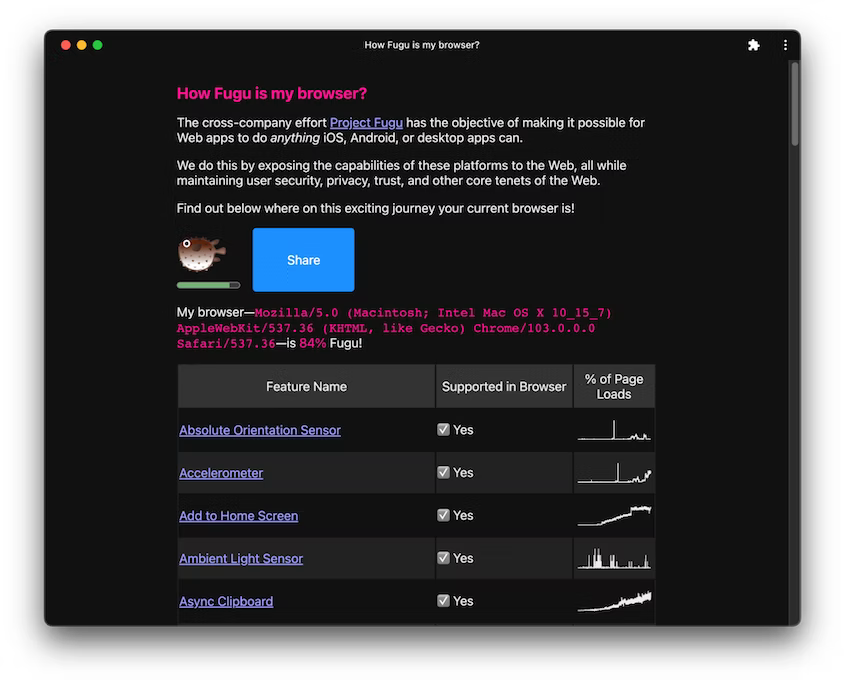
\includegraphics[width=0.9\columnwidth]{fugubrowser.png}
    \caption{The \textit{How Fugu is my browser?} app}
    \label{fig:fugubrowser}
    \Description{Screenshot of the How Fugu is my browser app.}
\end{figure}

\subsection{How Fugu is the Web?}

The companion browser extension named \textit{How Fugu is the Web?}\footnote{\url{https://goo.gle/how-fugu-is-the-web}} (see \autoref{fig:fuguweb}) will help you to find out which Fugu APIs are used by the sites you are visiting. Install this extension from the Chrome Web Store and browse the Web, then notice how the Fugu fish counter on some sites displays a~badge with the detected Project Fugu APIs. For example, if you browse to Excalidraw,\footnote{\url{https://excalidraw.com/}} the counter jumps to~9, since Excalidraw uses nine detectable Project Fugu APIs.

\begin{figure}[t]
    \centering
    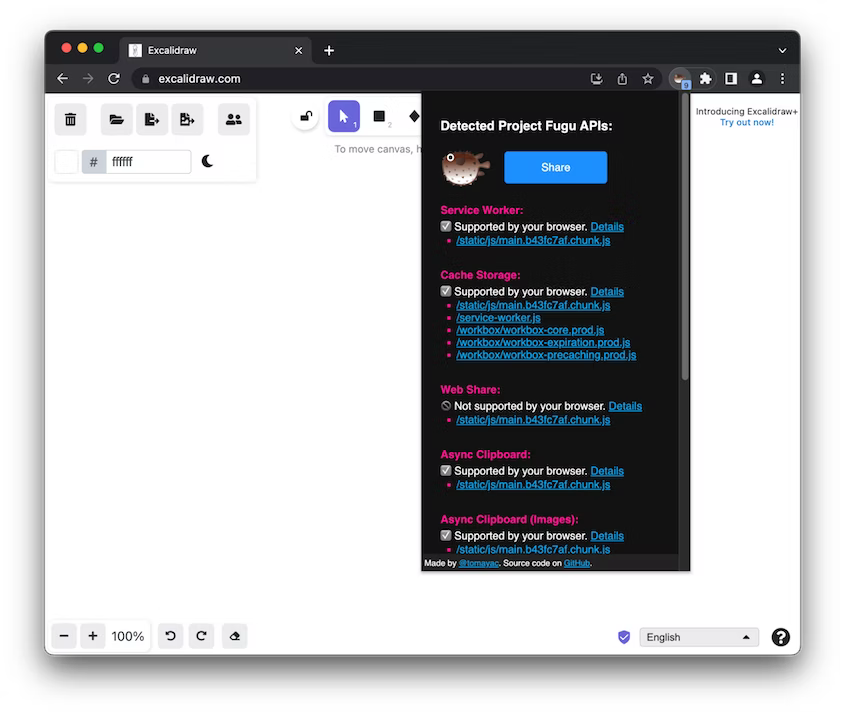
\includegraphics[width=0.9\columnwidth]{fuguweb.png}
    \caption{The \textit{How Fugu is the Web?} extension invoked on the site \url{https://excalidraw.com/}}
    \label{fig:fuguweb}
    \Description{Screenshot of the How Fugu is the Web extension invoked on the site excalidraw.com.}
\end{figure}

\section{Conclusions}

It's undeniable that amazing apps can be built on the Web. Photoshop, VS~Code, and Twitter are the stand-out examples in this paper, but there are many others.\footnote{\url{https://developer.chrome.com/fugu-showcase/}} One of the Web's super powers is its linkability, which is hard to beat on platforms other than the Web. There seems to be a~certain tendency for cross-platform app frameworks to become less attractive to developers, with the notable exception of Flutter, which allows for Web as one of its target platforms. Reasons for not building for the Web are easy to find, but it's also not hard to find counter-arguments to take these reasons apart. Some of them rely on outdated or weak assumptions, for example, PWAs not being welcome on app stores, or platform-specific apps being more secure than PWAs. Others are things that are in process, like closing the app gap by adding missing Web platform APIs. Some reasons apply equally to both worlds, for example, for hiring to be a~challenge. In this paper, I have given a~number of really strong arguments for building for the Web, while also not hiding the fact that the Web is a~platform that is still not perfect---yet incredibly capable, as \textit{How Fugu is the Web?} and \textit{How Fugu is my browser?} show---and pointing out that other alternatives exist. And as the three introductory app examples show, the decision is also not mutually exclusive. You can build a~powerful Web app, and have a~great, platform-specific application at the same time.
\end{document}
\endinput
